\documentclass[Dissertation.tex]{subfiles}
\begin{document}
\chapter{Dataset Exploration}\label{sec:dataEx}
\section{Introduction}
This chapter investigates the structure and content of the Brexit Blog Corpus, beginning with an informal description of the data followed by numerical and visual analysis. The chapter concludes with a brief note on the evaluation metrics used in the remainder of this project. 
\section{Dataset Description} \label{Data}

The dataset comprises 1,682 utterances  labelled for speaker stance according to a framework of ten notional categories of speaker stance \cite{simakiAnnotatingSpeakerStance2017}. The utterances are extracted from political blog posts related to the United Kingdom 2016 EU membership referendum. The manual annotation procedure in \cite{simakiAnnotatingSpeakerStance2017} is described as follows: two annotators from linguistics backgrounds were each asked to annotate each utterance with up to five of the ten notional stance categories. The annotators were also asked to repeat the process, in order that there be two sets of annotations from each annotator, allowing inter-annotator and intra-annotator agreement scores to be calculated. Where there was significant divergence between annotations, utterances were discussed by the annotators and final annotation was agreed upon. In Table \ref{tab:stanceExamples} are brief definitions of each stance category together with two sentences demonstrating each category.


{\renewcommand{\arraystretch}{2.5}
	\centering
	\begin{table}[]
		\caption{Stance categories, descriptions and examples}
		\label{tab:stanceExamples}
		
		\begin{tabularx}{\textwidth}{>{\raggedright}p{3cm} >{\raggedright}p{5.5cm} X}
			\toprule
			Stance Category        & Description                                            & Examples                                                                                                                                      \\ \midrule
			\small\scshape Agreement/ Disagreement &Utterance aligns with or against an opinion &\itshape That is the wrong approach. \par I believe this a good idea.\\
			\small\scshape Certainty              &Utterance shows conviction or confidence in statement& \itshape It is absolutely clear. \par Without a doubt this is possible.                                          \\
			\small\scshape Contrariety            & Utterance shows compromise or comparison               & \itshape Some think this is good, but others disagree.\par We have come far,  but there is still much to be done\\ 
			\small\scshape Hypotheticality        & Utterance describes consequences of a premise          &\itshape If that happened, it would be a disaster.\par I would be happy if he won.                              \\
			\small\scshape Necessity              & Utterance expresses an obligation or a request         & \itshape You must do it.\par I have to be there.                                                                \\
			\small\scshape Prediction             & Utterance shows speculation                            &\itshape The match should be an easy win.\par I think the journey will go by quickly.                           \\
			\small\scshape Source of Knowledge    & Utterance refers to the origin of opinion or statement & \itshape James told me he is moving house.\par The film was rated highly in the newspaper.                      \\
			\small\scshape Tact/Rudeness          & Utterance is either  polite or abrasive           & \itshape I would be grateful if you do this.\par I couldn’t give a damn how you feel.                           \\
			\small\scshape Uncertainty            & Utterance admits doubt                                 & \itshape To be honest I am not sure.\par I can’t guarantee I can make it.                                       \\ 
			\small\scshape Volition & Utterance  expresses desire or preference &  \itshape We wanted him to go to college. \par I wish you could visit us.\\
			\bottomrule
		\end{tabularx}

\end{table}}

Each example contains stance characterising elements of varying lengths. For example, {\small\scshape Necessity} can be expressed with individual stance markers such as \textit{must}, but also with longer phrases such as \textit{there is no other way}. It is important to note that the categories are not mutually exclusive, and utterances in the dataset can have multiple labels. Table \ref{tab:dataExtracts} shows several extracts from the data set, including utterances with multiple labels. Intuitively it can be seen that some stance markers relate to more than one category. For example, a sentence containing the stance marker \textit{I think} could be categorised as {\small \scshape Hypotheticality}, {\small \scshape Uncertainty}, or both. There are also natural relationships between categories. While hypothetical constructions inherently contain a prediction, Simaki~et~al. instructed annotators to label such instances as {\small \scshape Hypotheticality} only rather than {\small \scshape Hypotheticality} and {\small \scshape Prediction} \cite{simakiAnnotatingSpeakerStance2017}.


{\renewcommand{\arraystretch}{1.5}
	\centering
\begin{table}[]
	\caption{Dataset Extracts
	\label{tab:dataExtracts}}
	\begin{tabularx}{\textwidth}{>{\raggedright}X >{\raggedright \arraybackslash}p{5cm}}
		\toprule
		Utterance 											& Stance Categories \\ \midrule
		\itshape It might help us to solve some of the intractable problems in the world and start to move forward. &\small\scshape Uncertainty \\
		\itshape Under the Fixed-term Parliaments Act 2011, elections now take place every five years, unless an early election is triggered. &\small\scshape  Hypotheticality, Source of Knowledge \\
		\itshape Of course, this is far from the dominant narrative we hear in the media. & \small\scshape Agreement/Disagreement \\
		\itshape They’ll trade alright, but any post brexit EU trade agreement will have a stiff price attached as Norway will testify. &\small\scshape  Contrariety, Prediction\\
		\itshape Yes, we want worker protection, but we don’t need to go over the top as the EU does. & \small\scshape Necessity, Contrariety, Volition\\
		\itshape I’m glad that you stated your position so clearly in your last post. &\small\scshape  Tact/Rudeness
		 \\\bottomrule
		
	\end{tabularx}

\end{table}}

\section{Exploratory Data Analysis} \label{sec:EDA}
Before developing an experimental methodology and building classifiers, exploratory data analysis was undertaken to visualise the dataset and investigate its statistical properties.


\begin{figure}
	\centering
	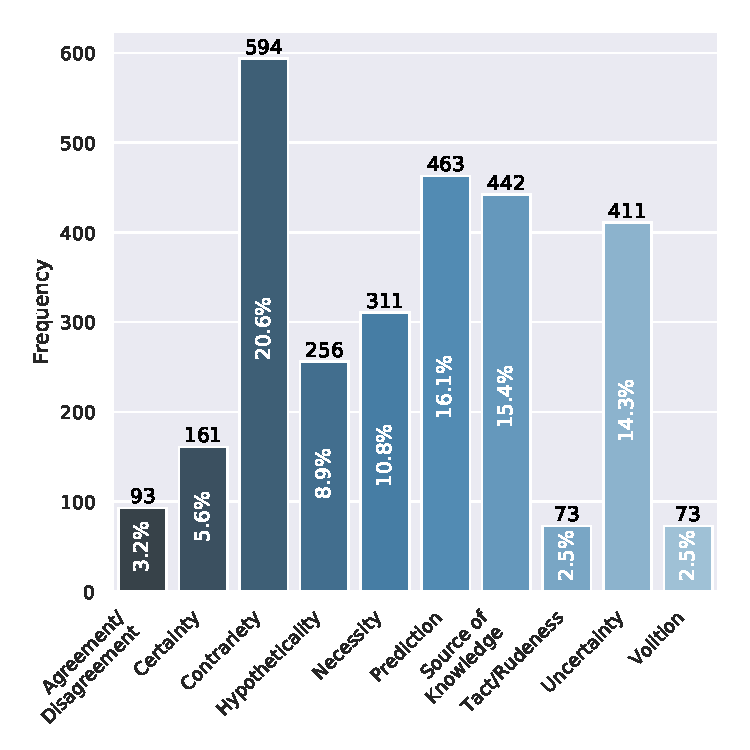
\includegraphics[width=4in]{label_counts.pdf}
	\caption{Bar chart of label counts}
	\label{fig:labelBarChart}
\end{figure}

Figure \ref{fig:labelBarChart} shows the distribution of labels in the dataset in a bar chart. From this we can see that the dataset is unbalanced. The most common labels are \lab{Contrariety, Prediction} and \lab{Source of Knowledge}, accounting for 52.1\% of labels.  The least common three labels are \lab{Agreement/Disagreement, Tact/Rudeness} and \lab{Volition}, accounting for just 7.9\% of labels.  Given that the dataset is fairly small, with only 1682 training instances, and in consideration of the class imbalances, it is expected that model performance could be diminished in classifying less frequent classes with less training data.


\begin{figure}
	\centering
	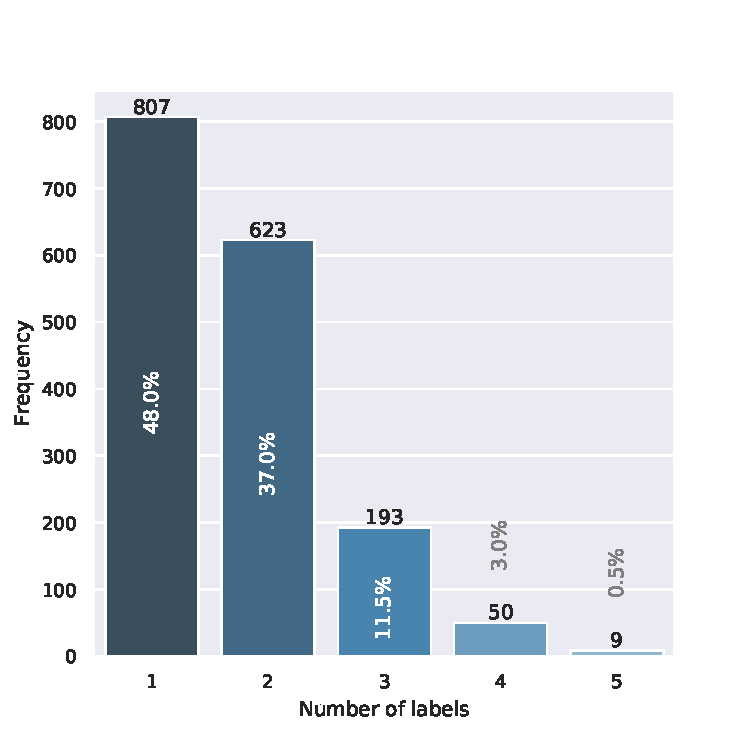
\includegraphics[width=4in]{num_labels.pdf}
	\caption{Bar chart of labels per instance}
	\label{fig:numLabels}
\end{figure}

In Figure \ref{fig:numLabels} is a frequency bar chart showing the  the number of labels associated with each utterance. With 85\% of the dataset comprising utterances labelled with up to two stance categories there is a clear bias towards fewer labels, and it is expected that most possible label combinations are not observed in the data. This can be measured by taking the label power set transform of the dataset (as described in Section \ref{sec:multiLabel}) and counting the number of unique labels. With the constraint of choosing up to five labels from a set of 10 the magnitude of the label powerset space $ |\mathbb{C}_{lp}| $ is given by:

\[ |\mathbb{C}_{lp}| = \sum_{k=1}^{k=5}\bigg( 		\begin{array}{c}
10\\
i
\end{array} \bigg) = \sum_{k=1}^{k=5}\frac{10!}{k!(10-k)!} = 637 \]


In fact, only 92 powerset labels are observed in the data, so there are only 92 stance category combinations in the Brexit Blog Corpus. Figure \ref{fig:polarBarChart} shows a log polar bar chart for power set label frequency, with the ten most common highlighted. Notably, none of the ten most frequent have more than two stance categories. The limited number of combinations observed in the data and the prevalence of utterances annotated with two stance categories or fewer suggests that there are underlying relationships between labels that could be exploited in modelling.
\begin{figure}
	\centering
	
	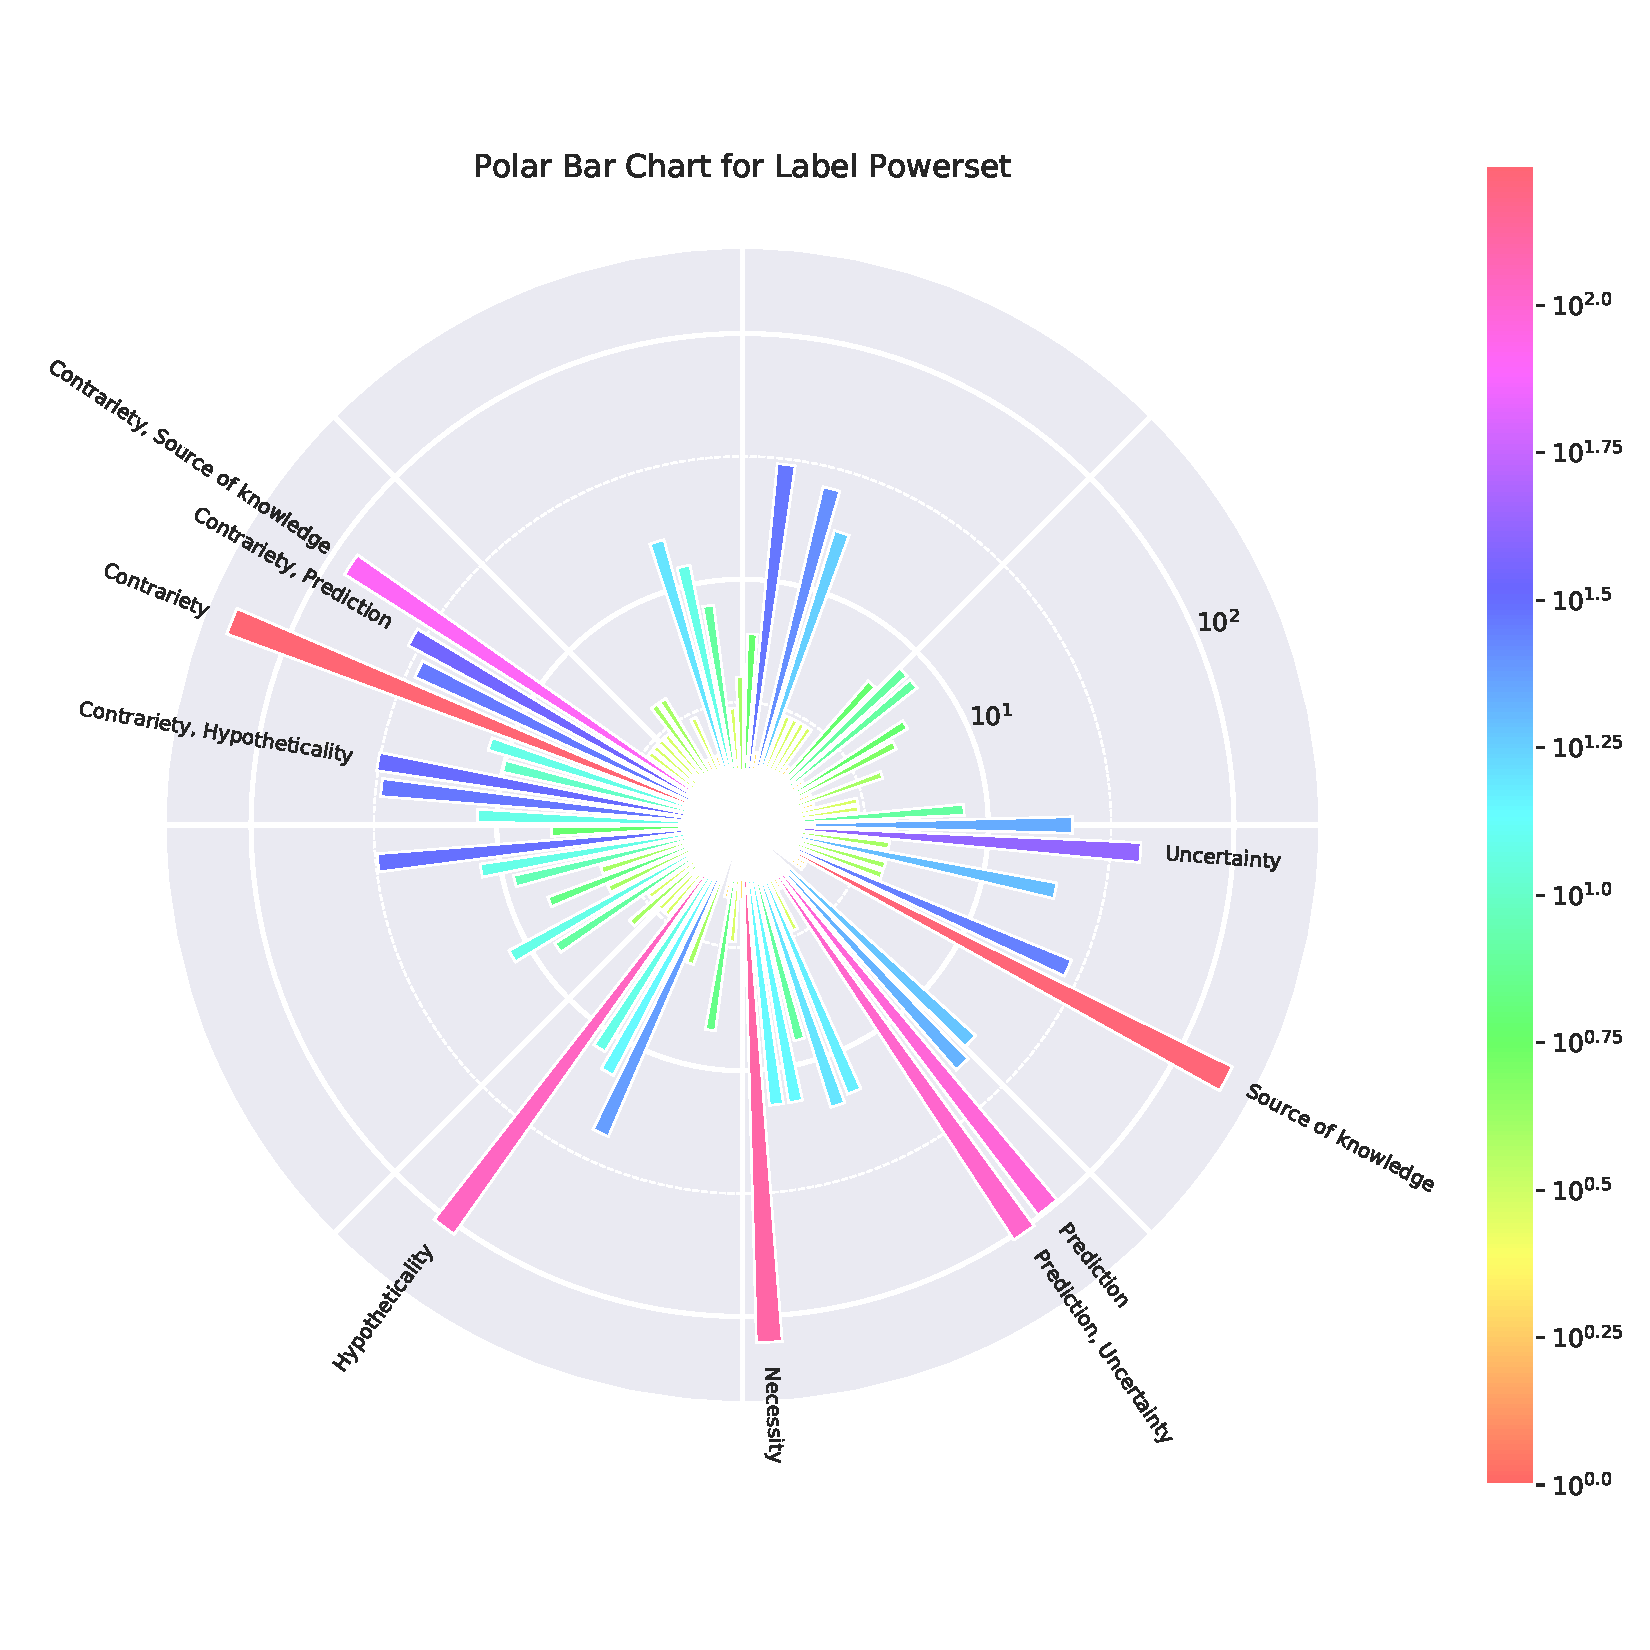
\includegraphics[width=7in]{label_powerset_polarplot.pdf}
	\caption{Log polar bar chart for label powerset}
	\label{fig:polarBarChart}
\end{figure}


In Table \ref{tab:labelFreq} shows per-category co-occurence statistics, with the following definitions: \begin{itemize}
	\item Total occurrences: Frequency with which a category occurs throughout dataset
	\item Co-occurrences: Frequency with which a category is jointly annotated with other categories
	
	\item Co-occurrence ratio: Ratio of co-occurrences against total occurrences
	\item Mean co-occuring labels: Mean number of labels jointly annotated with a category
	\item  STD co-occurring labels: Standard deviation of labels jointly annotated with a category
\end{itemize}

\begin{table}
	\caption{Label co-occurence statistics}
	\label{tab:labelFreq}
	\subfile{../tables/label_frequency_and__co_occurence.tex}
	
\end{table}

From Table \ref{tab:labelFreq} it can be see that \lab{Hypotheticality} exhibits the largest co-occurrence ratio at $ 0.43 $, suggesting that hypothetical constructs frequently include or appear together with stance markers for other categories. Interestingly, \lab{Uncertainty} shows the highest mean co-occurring labels despite having the lowest co-occurrence ratio. This suggests that though constructs of uncertainty rarely occur jo	intly with other categories, those which do are associated with a broad range of other categories. \lab{Volition} has the highest standard deviation of co-occurring labels. This could be explained by an underlying trend, however this may also be explained by small sample size since there are only $ 73 $ total occurrences of \lab{Volition} in the data..

Figure \ref{fig:labCoOc} shows a label co-occurrence heatmap of the dataset. While the co-occurences are somewhat skewed due to imbalances in the data, there are several notable features to the plot. \lab{Contrariety} stands out as most frequently co-occurring category,  and is particularly related to \lab{Source of Knowledge} and \lab{Uncertainty}.	 There are also several other clear correlations between category pairs, such as between \lab{Uncertainty} and \lab{Prediction}, and between \lab{Hypotheticality} and \lab{Uncertainty}.


\begin{figure}
	\centering
	\hspace*{1em}
	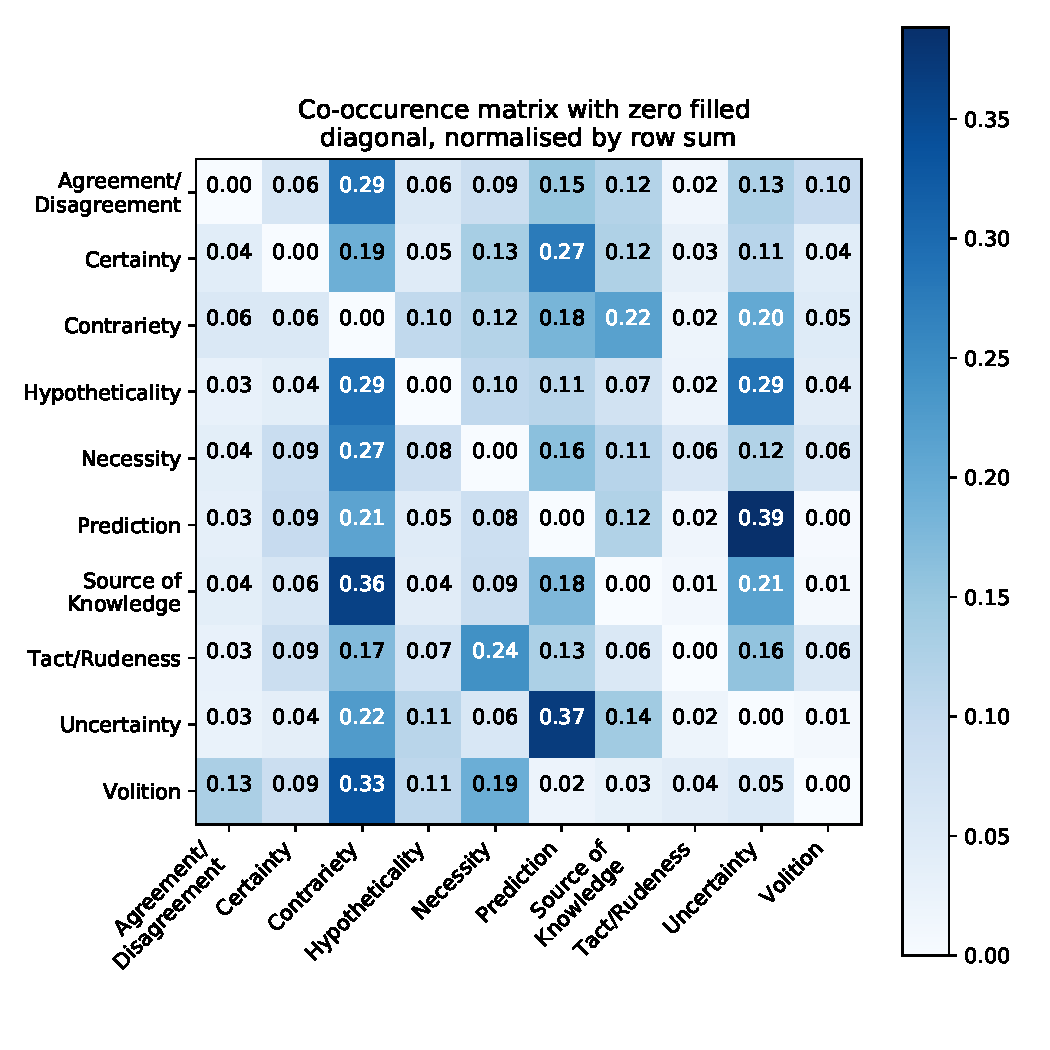
\includegraphics[width=5in]{label_confusion_matrix.pdf}
	\caption{Label co-occurence matrix heatmap}
	\label{fig:labCoOc}
\end{figure}




\subsection{Metrics for Evaluation}
In any data science project, choosing appropriate metrics for evaluation is of utmost importance. This can help to ensure realistic goals are set out, but also  safeguards against over or underestimating performance. This is particularly true when using multi-label data since many conventional metrics become ambiguous or are undefined in multi label domains. In single label data, common evaluation metrics are \textit{Accuracy, Precision, Recall} and \textit{F\textsubscript{1}-measure} \cite{sorowerLiteratureSurveyAlgorithms2018}. All of these metrics rely inherently upon a binary evaluation of each prediction as \textit{correct} or \textit{incorrect} \cite{sorowerLiteratureSurveyAlgorithms2018}. However, since in multi label problems the target variable is a set of labels, a prediction can be \textit{completely correct}, \textit{partially correct}(to varying extents) or \textit{completely incorrect}. Single label evaluation measures cannot capture this ambiguity, and so other metrics must be chosen.

A possible approach is to simply ignore partially correct results, mark them as completely incorrect and calculate accuracy. This is known as the \textit{Exact Match Ratio} (EMR) \cite{sorowerLiteratureSurveyAlgorithms2018}. While this can be useful, this is a harsh metric.

A notable important conclusion of the data analysis in the so far is the imbalance in stance categories present in the dataset. In single label domains, class imbalance is usually accounted for by evaluating performance based on F-measure, which is defined as the harmonic mean of precision and recall \cite{sorowerLiteratureSurveyAlgorithms2018}. F\textsubscript{1}-measure can be modified to evaluate multi label problems. Multi label F\textsubscript{1}-measure is therefore defined as \cite{sorowerLiteratureSurveyAlgorithms2018}:

\[ F_1 = \frac{1}{n}\sum_{i=1}^{n}\frac{|\mathbf{y}_i \cap \mathbf{\hat{y}}_i|}{|\mathbf{y}_i|}\] 

Where $ \mathbf{y} $ is the set of correct labels and $ \mathbf{\hat{y}} $ is the set of predicted labels. F\textsubscript{1}-measure can also be calculated in the conventional manner for each category as if it were a binary classification, which is here after termed categorical F\textsubscript{1}.


To summarise, there exist several evaluation methods that are applicable to multi-label datasets. Due to the imbalances present in the Brexit Blog Corpus micro F\textsubscript{1} and macro F\textsubscript{1} are the primary evaluation metrics in this project. EMR is considered as secondary metric while categorical F\textsubscript{1} is used only for multi-task and multi-label models, since calculation of F\textsubscript{1} for the ten stance categories is not possible in the multi-class models. 

\end{document}